\documentclass[conference,10pt]{IEEEtran}
% Re-allow e.g. the \thanks command.
\IEEEoverridecommandlockouts

% to be able to draw some self-contained figs
\usepackage{tikz}
\usepackage{amsmath}
\usepackage{minted}
\usepackage[utf8]{inputenc}
% \usepackage{todo}
\usepackage{csquotes}
\usepackage{amsthm}
\usepackage{siunitx}
\usepackage[caption=false]{subfig}
\usepackage{listings}
\lstset{
  basicstyle=\scriptsize\ttfamily,
  mathescape=true,
  %numbers=left,
  aboveskip=\medskipamount,
  belowskip=\smallskipamount,
  numberstyle=\tiny,
  %stepnumber=2,
  numbersep=10pt,
  tabsize=2,
  extendedchars=true,
  breaklines=false,
  keywordstyle=\color{black}
  }
\newcommand{\lstcd}[1]{\lstinline[basicstyle=\ttfamily\small]{#1}}

% this style is used for long/verbatim notes (not text) in the paper
\lstdefinestyle{meta}
  {basicstyle=\tiny\ttfamily\color{magenta}}

\usepackage{hyperref}
\usepackage[capitalise]{cleveref}
  % i.e., you use '\cref{x}' rather than "Figure \ref{x}"
% inlined bib file
\usepackage{filecontents}

% SYSTEM OF ANNOTATIONS:
\newcommand{\info}[1]{\textcolor{blue}{[[#1]]}}
\newcommand{\note}[1]{\noteYes{#1}}  
\newcommand{\noteNo}[1]{}  % way to remove all notes.
\newcommand{\noteYes}[1]{\textcolor{red}{[[#1]]}}
\newcommand{\todo}[1]{\note{TODO: #1}}
\newcommand{\todoa}[1]{\todo{[\#A]: #1}}
\newcommand{\todob}[1]{\todo{[\#B]: #1}}
\newcommand{\todoc}[1]{\todo{[\#C]: #1}}
\newcommand{\old}[1]{\textcolor{orange}{[[OLD: #1]]}}


\newcommand{\paragraphsection}[1]{\vspace{7pt}\noindent{\textit{#1}}}
  % use this for "Initial Results" or for sections at the lowest level.
  % TODO: is the formatting sufficiently smaller than level 2 sections?
 
\sisetup{group-separator={,}, group-minimum-digits=4}

\begin{document}

\date{}

% make title bold and 14 pt font (Latex default is non-bold, 16 pt)
\title{Strengthening Weak Links in the PDF Trust Chain}

\author{
    \IEEEauthorblockN{ Mark Tullsen, William Harris}%
    \IEEEauthorblockA{\small Galois, Inc.\\
    \texttt{\{tullsen,wrharris\}@galois.com}} \and
    \IEEEauthorblockN{Peter Wyatt}
    \IEEEauthorblockA{\small PDF Association\\
    \texttt{peter.wyatt@pdf.org}}
}

\maketitle

%-------------------------------------------------------------------------------
\begin{abstract}
%-------------------------------------------------------------------------------

\todo{WRITE ABSTRACT...}
  
\end{abstract}

\section{[Meta-Notes for Authors]}

\begin{lstlisting}[style=meta]
CONVENTION:
 - using this lstlisting[style=meta] environment to capture
   text in outline form that has not been fleshed out / turned into prose.
\end{lstlisting}

\begin{lstlisting}[style=meta]
META NOTES:  
- shoot for 12 pages
- challenge: figuring out how much detail to go into, e.g., xref
- the idiom
  - details (e.g., in PDF)
  - general principles
    - E.g., such as
      - cavities
      - trust-chain 
      - redundant-data [highlight]
        - E.g., Size, we don't want to *invisibly*
          null-out obj. nums > Size
      - file-offsets in format
      - schizophrenia / polyglot
      - limitations of informal (english) standards
   - at least 1 other example of the principle
   - ICC, etc.
TERMS (to actually use, and define when needed):
- complies with standard, compatible with standard
- Pre-DOM
- ?? for the repetitious use of ``parsing and computation''
\end{lstlisting}

% ------------------------------------------------------------------------------
\section{Introduction \note{1.5pp}}
\label{sec:intro}

\subsection{PDF and its challenges}
\label{sec:pdf-challenges}

\begin{lstlisting}[style=meta]
- Creation of DOM ("document object model")
  - list of object definitions
  - ... containing object references
  - designated root object
- Cross-reference (xref) table
  - table with byte offset for each object
- Cross-reference streams (added in PDF 1.5) [7 pp. in spec]
  - compressed, complicated, space-efficient, ...
  - allows for hybrid files with both traditional
    xref tables and new xref streams
- Incremental updates
  - by only appending to PDF file we can add, update, delete, restore objects
- Linearized PDF (efficient incremental access) a.k.a. "Fast web view"
  - "differential by design"!
\end{lstlisting}

\begin{lstlisting}[style=meta]
- We must accurately create the DOM (a DAG, no cycles allowed)
  - ... while abstracting over xref tables, xref streams,
    hybrid files, incremental updates, linearization
  - ... while recovering from errors
  - ... while doing xref table reconstruction

- This is the source of errors, ambiguities, and vulnerabilities!
\end{lstlisting}

\subsection{PDF Vulnerabilities}
\label{sec:pdf-vulnerabilities}
\todo{here, briefly describe vulnerabilities, citing the literature,
  but not going into great detail.
  In \cref{sec:predom-vulnerabilities}
  we'll go into further detail on pre-DOM vulnerabilities.
}

\begin{lstlisting}[style=meta]
- Schizophrenic files
- Polyglot files
- [QUESTION: these last two common terms or ``Safedocs''-isms?]
- Shadow attacks: possible because of ability to sign dead objects and cavities
- Steganographic attacks (similar to Shadow)
- Multiple places for hidden/unused/malicious data in PDF
  - non-obvious places, unnoticed when "simply parsing"
  - e.g., shadow-attacks
  - dead bytes, dead objects, dead updates, dead linearization sections, etc.
\end{lstlisting}

\todo{Refer to these and others:
  pdf-insecurity.org publications,
  https://itextpdf.com/en/blog/technical-notes/investigating-pdf-shadow-attacks-depth-pdf-security-using-itext-part-3,
  K. Koptyra and M. R. Ogiela, “Distributed Steganography in PDF Files - Secrets Hidden in Modified Pages,” Entropy, vol. 22, no. 6, p. 600, May 2020, doi: 10.3390/e22060600.
}

\subsection{Summary of Paper}

\todo{in section 1 we ... blah, in section 2 blah, ... [Mark hates writing this useless paragraph]}

% ------------------------------------------------------------------------------
\section{The PDF Trust Chain \note{1.5pp}}
\label{sec:trust-chain}

What do we mean by the term ``PDF Trust Chain'' in our title?

\subsection{Trust Chains}

The term \emph{Trust Chain} is used in multiple contexts, e.g.,
\emph{digital certificates}: a sequence of certificates signing certificates,
starting with a root certificate;
\emph{supply chain}: a product is no more reliable or secure as its
outsourced components;
\emph{trusted boot}: unless the bootloader is correct and non-malicious,
there can be no possibility of the operating system being the same;
\emph{software stacks}: upper layers are dependent upon lower layers (such as
system libraries) and vulnerabilities at the bottom affect all layers above.

The common idea is that we have layers/components that rely on lower
layers/sub-components/etc for their validity.
And the key lesson being,
{\bf{if a single element of the trust chain 
  is flawed or suborned, then every element ``above'' it
  is no longer capable of being trusted.}}


\subsection{The Trust Chain Inside PDF Parsers}

% In \cref{sec:pdf-challenges}, we elaborated on the challenges of PDF.
% Parsing data-formats has a long history and many solutions ...
% Parsing formal languages also has a long history and many solutions ...
% PDF has aspects of both: this makes PDF challenging.
% But PDF ``parsing'' is not merely a matter of harder [difference of degree]
% but intrinsically more complex [a difference of kind!]:

\begin{figure}[t]
    \centering
    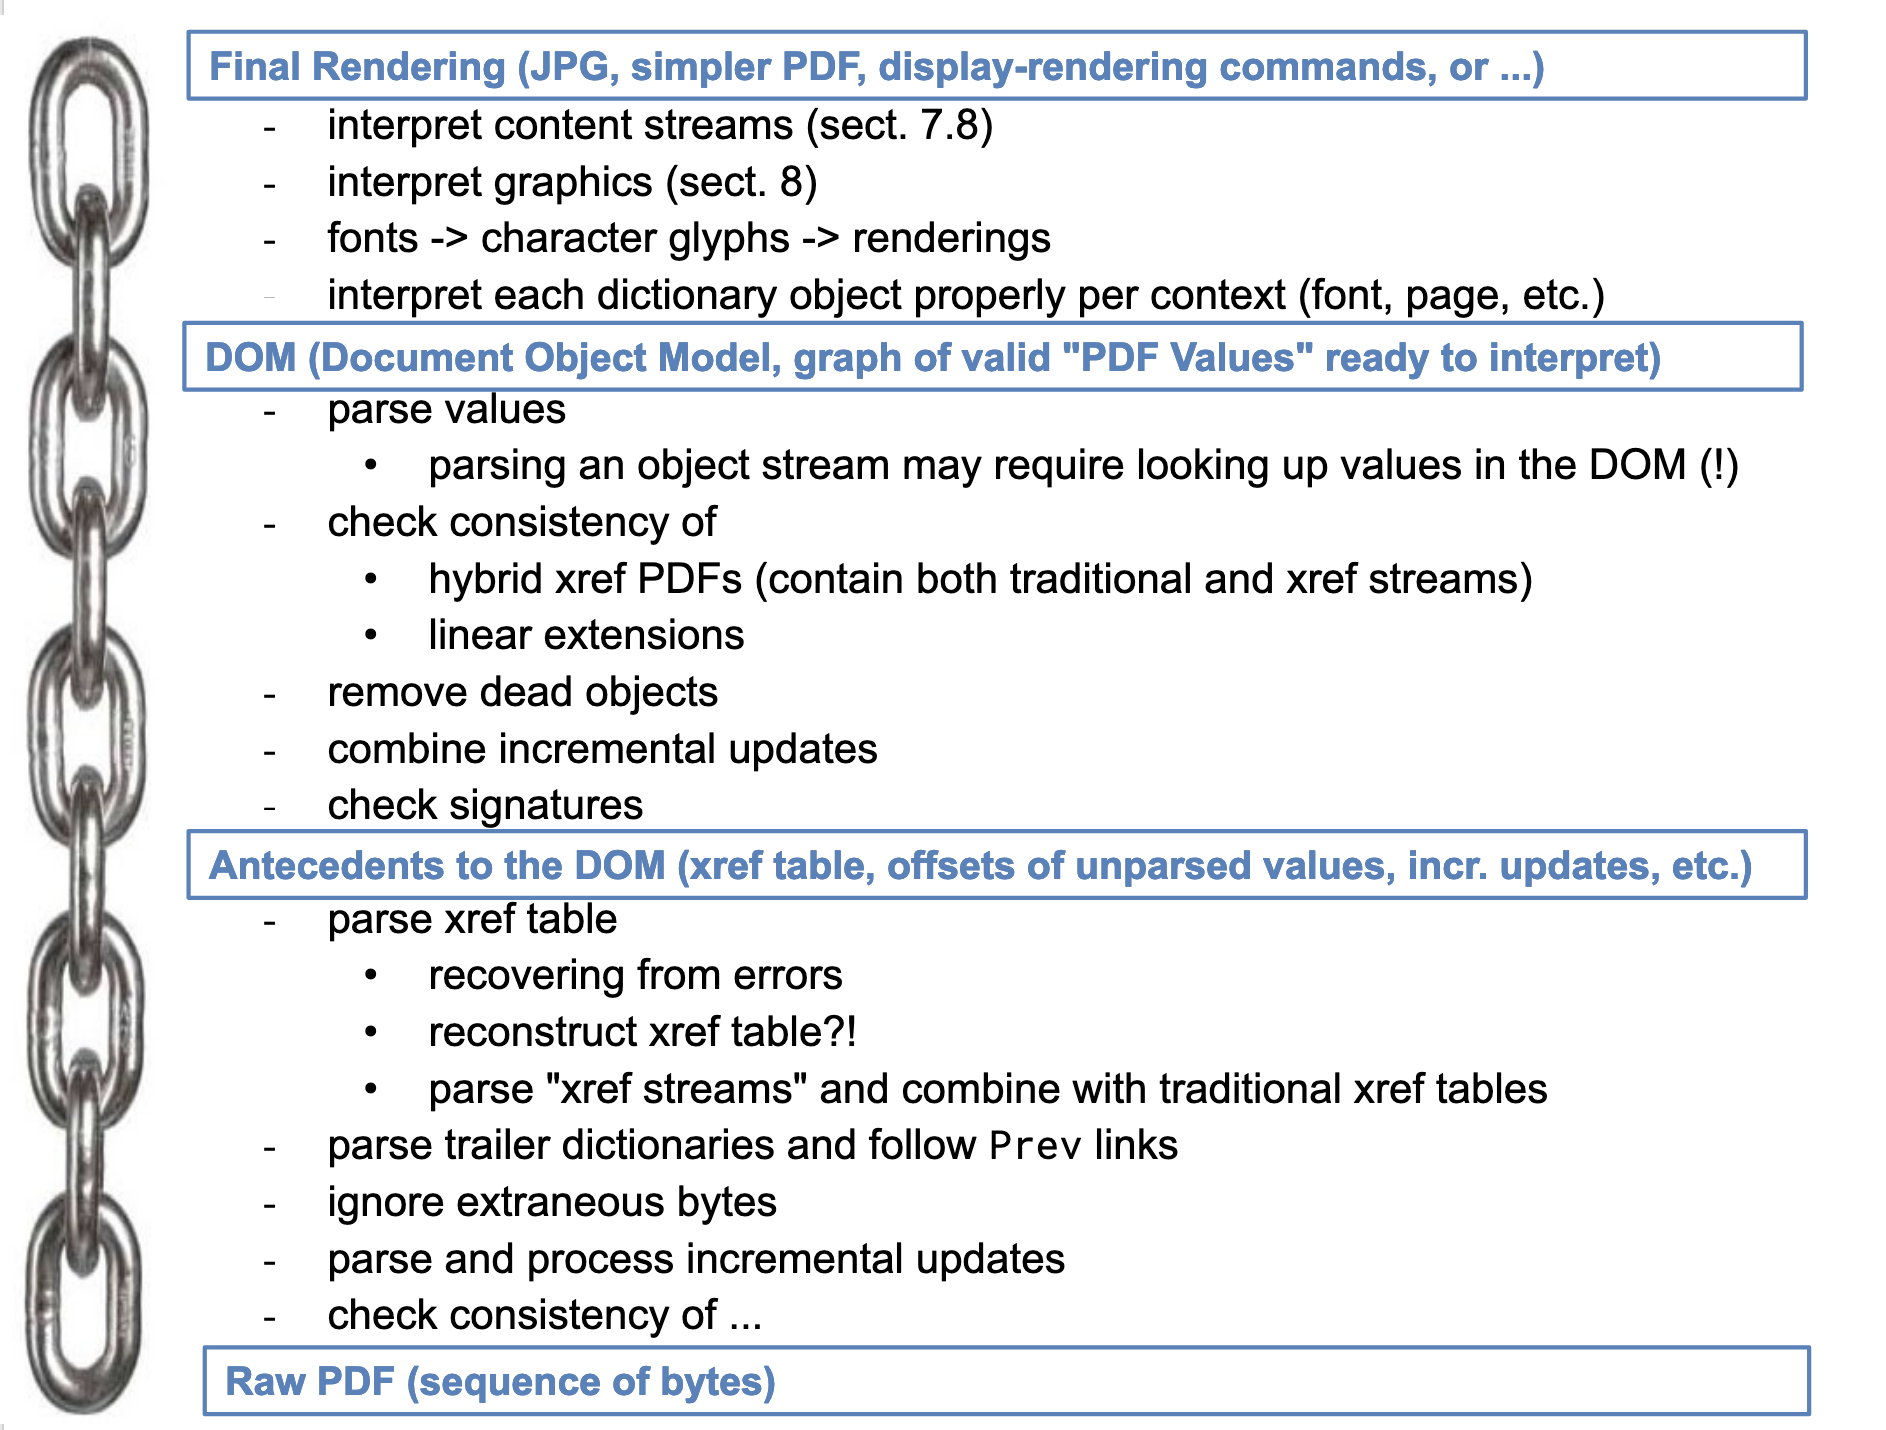
\includegraphics[width=\linewidth]{figures/trustchain-diagram.png}
    \todo{revamp diagram - please add "phase" initiate processing = seek to EOF, locate startxref keyword, etc.}
    \caption{The PDF Trust Chain diagramed.}
    \label{fig:pdf-trust-chain}
\end{figure}

In \cref{sec:pdf-challenges} we touched upon the complexities of parsing
PDF, but to appreciate these, one has to understand the
dependencies and interactions between the \todo{features/aspects/?}.
In \cref{fig:pdf-trust-chain} we attempt to show these diagrammatically.
\todo{explain the [reworked] diagram ...}

% between the ``phases'' of the parsing process.

The attentive reader will note that we have another instance of a \emph{Trust
Chain}.  The later phases of the parsing process are \emph{completely
dependent} upon the earlier phases to properly parse and interpret the PDF
file.

% The PDF "trust chain": higher levels of abstraction depend upon lower levels.
% These structures are not necessarily concrete values--e.g. parsed xref
% table--but they do exist `conceptually'.

We think understanding a PDF parser in terms of this \emph{Trust Chain} is
important:
%
(1) it highlights the presence of the many ``dependent'' parsers (or phases)
in PDF processing.
%
(2) it highlights the importance of ensuring the pre-DOM parsing and
computation (the base of our Trust Chain) is correct and secure.
%
(3) it reminds us that the integrity of the DOM cannot be verified
independently of the lower levels.

\todo{introduce terms such as Pre-DOM}
\todo{say ... regarding our repetitious use of ``parse and compute''}
    
% ------------------------------------------------------------------------------
\section{Pre-DOM Vulnerabilities \note{2.5pp}}
\label{sec:predom-vulnerabilities}

As will become even more apparent, there is a significant amount of
parsing and computation that needs to be done \emph{pre-DOM}.
And given our recent points about the \emph{PDF Trust Chain}
(\cref{sec:trust-chain}),
it should not surprise us that most of the PDF attack vectors
(\cref{sec:pdf-vulnerabilities})
involve some aspect of breaking the \emph{DOM} abstraction.
I.e., they occur at the \emph{pre-DOM} levels.

\todo{notion of cavities [belongs?]}

{\bf{Shadow Attacks}} \todo{...}

{\bf{Schizophrenia}} \todo{...}
\begin{lstlisting}[style=meta]
  - writer errors
  - parser differentials
    - e.g., ignoring xref tables
  - recovering parsers !!
  - blind faith in incremental updates (Shadow Attacks)
\end{lstlisting}

{\bf{Polyglots}} 
\todo{... arising from cavities and permissive implementations and ...}

{\bf{Denial of Service (DOS)}} 
%
\begin{lstlisting}[style=meta]
- [potential recursion many places]
- format may not be well-defined because the recursion is not
    "well-defined"
\end{lstlisting}

{\bf{Others}} \todo{have any others here??}

% ------------------------------------------------------------------------------
\section{Securing the Pre-DOM Components \note{1pp}}
\label{sec:securing}

There are four primary approaches we are taking to improve the security of the
Pre-DOM components of PDF parsing:
\begin{enumerate}
\item
  \emph{Develop tools for inspection and validation of pre-DOM structures.}
  We have developed a tool that ..., this tool validates more of the structure
  than ... .  Using it we can find dead objects and cavities.
  This tool is open source and can be found as part of the Daedalus
  project \cite{daedalus-url}.
 
\item
  \emph{Understand and clarify the PDF standard.}
  In the process of doing the above, we have pushed the bounds
  of our PDF knowledge and have discovered multiple places in which
  the PDF specification is ambiguous or could be made more clear.
  We have also found instances in which the specification
  does not correctly specify a well-defined parseable format:
  \todo{examples being ...}
  ... or in which the intentions of the committee was not made clear in
  the spec.
  
\item
  \emph{Write a formal specification for pre-DOM processing.}
  Wanting to formally capture what we have learned in 2 ...
  The ISO Standard PDF 2.0 Specification \cite{isotc171sc2wg8ISO32000220202020}
  is English, not ``formal'',
  unclear in places, \todo{...}
  (see \cref{sec:specifying}).
  
\item
  \emph{Analyze Extant Data}
  \todo{...}
  
\end{enumerate}

In this paper we won't go into further details of our tool (1).
The work done with respect to (4) is discussed further
in \cite{icarus1,icarus2}.
  % I.e., the papers from Galois & other TA1 groups.
The lessons learned in (2)
have been captured in our specification (3) as much as possible.
Thus, the remainder of our paper will be going into much greater detail of
our specification.

% ------------------------------------------------------------------------------
\section{Specifying pre-DOM Components \note{4pp}}
\label{sec:specifying}

\subsection{[Motivating Specification]}
% REMEMBER: [terms: complies with standard, compatible with]

\begin{lstlisting}[style=meta]
- an implementation
  - should follow the standard
  - should safely support less than standard
  - pragmatically support some common extant data malformations
  - should carefully support more than the standard
  - should not "inf. loop"
    - lots of opportunities - failure to notice digitally signed PDFs that have been tampered! 
      - elaborate?
\end{lstlisting}

\begin{lstlisting}[style=meta]
- Lack of formality in standard. Thus, implementations:
  - are more effort
  - over implement, under implement, wrongly implement
  - backwards and forwards compatibility
  - "backwards parsing"
  - some requirements will not be checked by PDF readers ("writer only" file requirements) 
  - patch existing vs implement from scratch
- No definition of acceptable, reasonable error recovery
- Less than ideal design that reflects 27 years of an evolving standard
- Pre-DOM processing
  - is where many parsing errors & recovery occur
  - is non-trivial
  - involves multiple interdependent features and subtle dialects
  - involves multiple redundant features
    - schizophrenic if these features aren't mutually consistent
\end{lstlisting}

\subsection{The pre-DOM constructs}
\todo{Hmmm: how much detail to go into?
      How will reader understand next section if we say nothing?
}

\subsection{Specifying pre-DOM components}
\begin{lstlisting}[style=meta]
- presented
- going into PDF details, as needed (this section or separate section?)
\end{lstlisting}

% ------------------------------------------------------------------------------
\section{Conclusion \note{1.5pp}}
\label{sec:conclusion}

\subsection{Contributions}

As we discussed in \cref{sec:securing} we have ...

\todo{prosify the following bullet points, split into done/future.}

PDF pre-DOM parsing and semantics:
Clarified aspects of PDF with respect to incremental updates, minor parsing details
Submitted a problem in the definition of cross reference streams
(\cite{isotc171sc2wg8ISO32000220202020} Sec 7.5.8) to
ISO via Peter Wyatt.

Write a proposed implementation/specification for dealing with parsing (DOM-dependent) object streams
Develop formal definitions for pre-DOM parsing/computation

Tool for inspecting and checking PDF at the pre-DOM level:
Created tool for exploring the DOM Antecedent structures as well as validating
them (more than a PDF reader necessarily does).

Based on Galois's \todo{TA2} PDF parser, this tool can
parse and validate each incremental update separately
display "incremental updates," "incremental xref tables," parsed objects, and cavities (bytes that are not used)
validate that object definitions do not overlap (in their source bytes)
      
\subsection{Related Work}

\todo{pdf-hsdriver} 
\todo{Daedalus}
\todo{shadow attacks}

\subsection{Applications to Other Formats}

\todo{...}

\subsection{Future Work}
\todo{...}

Add more features to our tool and specification:
\begin{lstlisting}[style=meta]
- support linearized files (to improve cavity detection)
- more consistency checks: e.g, for hybrid xref files
- analysis and categorization of cavities
\end{lstlisting}

% ------------------------------------------------------------------------------
\section*{Acknowledgements}

This research was supported by the SafeDocs program under HR0011-19-C-0073 and HR001119C0079.
\todo{check these!}

% ----------------------------------------------------------------------------
\bibliographystyle{plain}

\bibliography{zotero-pdf-biblio,old,local}
  % zotera-pdf-biblio.bib
  %   The Zotero export (using Better BibTex Addon) of the PDF collection
  % old.bib
  %  - TA1's last LangSec paper
  % local.bib
  %  - all other references here

\end{document}
